%-------------------------------------------------------------------------
\documentclass[authoryear,preprint,review,12pt]{elsarticle}



%\setlength{\parskip}{1em}			% espaciar parrafos
\newtheorem{proposition}{Proposition}
\newtheorem{definition}{Definition}
\newtheorem{proof}{Proof}
\newtheorem{corollary}{Corollary}

\usepackage{hyperref}				% enlaces en el pdf
\hypersetup{colorlinks=true}	    % colores en vez de cajas en los enlaces
\usepackage{times}              	% la letra
\usepackage{graphicx}           	% para manejar imagenes
\usepackage{tabularx}		   		% para ajustar el ancho de las columnas
\usepackage{algorithm}				% Para el seudocódigo
\usepackage{setspace}				% Para el seudocódigo
\usepackage{amsmath}				% Para el seudocódigo
\usepackage[noend]{algpseudocode}	% Para el seudocódigo
\usepackage{multicol}				% Para el seudocódigo

% Change algorithm input/output
\renewcommand{\algorithmicrequire}{\textbf{Input:}}
\renewcommand{\algorithmicensure}{\textbf{Output:}}

\newcolumntype{L}[1]{>{\raggedright\let\newline\\\arraybackslash\hspace{0pt}}m{#1}}
\newcolumntype{C}[1]{>{\centering\let\newline\\\arraybackslash\hspace{0pt}}m{#1}}
\newcolumntype{R}[1]{>{\raggedleft\let\newline\\\arraybackslash\hspace{0pt}}m{#1}}

\begin{document}
	
	\title{A New Algorithm for Reduct Computation based on Gap Elimination 
		   and Attribute Contribution}
		
	
	\address{Computer Science Department\\
	Instituto Nacional de Astrof\'{\i}sica, \'{O}ptica y Electr\'{o}nica\\
	Luis Enrique Erro \# 1, Santa Mar\'{\i}a Tonantzintla, Puebla,
	72840, M\'{e}xico} 
	
	\begin{abstract}
		Attribute reduction is a key aspect of Rough Set Theory.  Finding the complete set of reducts is important for solving practical problems such as the assessment of attribute relevance, multi--objective 		cost--sensitive attribute reduction and dynamic reduct computation. The main limitation in the application of Rough Set methods is that finding all reducts of an information system has exponential complexity regarding the number of attributes. Several algorithms have been reported to reduce the cost of reduct computation. Unfortunately, most of these algorithms relay on operations for candidate evaluation with a high cost. Therefore, in this paper we propose a new algorithm for computing all reducts of an information system, based on the pruning properties of \textit{gap  elimination} and \textit{attribute contribution}, by using binary cumulative operations in order to reduce the algorithm runtime. Finally, the proposed algorithm is evaluated and compared against other state of the art algorithms, over synthetic and standard information systems.
	\end{abstract}
	
	\begin{keyword}
		Rough Sets\sep Reduct Computation\sep Typical Testor.
	\end{keyword}

	\maketitle

%-------------------------------------------------------------------------------
% your earth-shattering contribution

\section{Introduction}
% BAsico sobre los reductos
  Rough Set Theory (RST), proposed by Z. Pawlak in 1981 \citep{Pawlak81,Pawlak81-2,Pawlak82,Pawlak91}, 
  is a relatively new mathematical theory to deal with imperfect knowledge, in particular with vague 
  concepts. Into RST, information systems are tables of objects (rows) described by a set of attributes (columns). 
  When data is collected or recorded, every single aspect (attribute) of the objects under study is considered 
  to have a complete representation and to ensure that no potentially useful information is lost.
  As a result, information systems are usually characterized by a large number of attributes,
  which degrades the performance of machine learning tools \citep{Parthalain08}.
  One of the main concepts in RST is the notion of reduct, which is a minimal subset of attributes 
  preserving the discernibility capacity of the whole set of attributes \citep{Pawlak91}.  
  However, the main restriction in practical applications of RST is that computing all reducts of an 
  information system is NP--hard \citep{Skowron92}. 
  
%  Most of the work on reduct computation has been devoted to finding a single optimal reduct (having the minimum 
%  number of attributes) or a reduced number of reducts. Several heuristic approaches search for a pseudo optimal
%  reduct using a determined measure \citep{Zheng14,Liang2014}. Some stochastic approaches including Genetic
%  Algorithms \citep{Feng2012,Hedar2015}, Ant Colony Optimization \citep{Jensen03,Chebrolu2015} and Particle Swarm 
%  Optimization \citep{Chen15,Luan2015} have been also reported in order to achieve a better global optimization. 
%  In this paper, on the other hand, 
  %We are focused on solving the problem of computing all reducts of an information system. 
  Early algorithms for computing the complete set of reducts \citep{Bazan2001,Ohrn00} are integrated in RSES and ROSETTA software for rough sets computation. However, these algorithms are unable to solve even middle size problems \citep{Lazo15}. The divide and conquer approach presented by \cite{Starzyk99,Starzyk00}, and later modified in \citep{Jensen14}, operates over the binary discernibility function, which leads to inefficient data representations. A faster algorithm based on several properties for pruning the search space is proposed by \cite{WangP07}. This is a very efficient algorithm, nevertheless, its main drawback is that it works directly over the information system instead of the discernibility matrix.   
     	
% Relación con los testores
  RST reducts have been related to Typical Testors (TT) from the logical combinatorial approach 
  to pattern recognition \citep{Chikalov2013}. Testor Theory was originally created by \cite{Cheguis55} as a tool
  for analysis of problems connected with control and diagnosis of faults in circuits. 
  However, Testor Theory has been extended in order to be used for feature selection as shown in \citep{Dmitriev1966}, \citep{Martinez01} and \citep{Ruiz08}. Algorithms for typical testor computation can be applied to reduct computation due to the similarity between these two concepts \citep{Lazo15}. There have been developed two kinds of algorithms for computing typical testors: \emph{internal scale} algorithms, such as CT \citep{Bravo83}, CC \citep{Aguila84} and YYC \citep{Alba14}; and \emph{external scale} algorithms, such as BT and TB \citep{Ruiz85}, LEX \citep{Santiesteban03}, CT\_EXT \citep{Sanchez07} and BR \citep{Lias09}. The former approach analyzes the discernibility matrix to find out some conditions to guarantee that a subset of attributes is a typical testor. The latter, searches for typical testors by evaluating subsets of attributes over the power set, avoiding unnecessary evaluations by pruning some attribute subsets. Internal scale algorithms usually evaluate less candidates than external scale algorithms but each candidate evaluation has a higher computational cost. Therefore, the search for fast algorithms for computing typical testors has been biased to external scale algorithms \citep{Alba14}.
    
% Utilidad de todos los reductos
%  Although most algorithms for reduct computation search for a single reduct or a small subset of reducts, 
  The complete set of reducts of an information system is useful for solving some practical problems and real--world applications. \cite{Xu2013} developed a multi-objective cost-sensitive attribute reduction. First, they compute all reducts of an information system. Then, they separately calculate the cost, in terms of time and money, of every reduct. Finally, the worst reducts are dismissed, leaving a Pareto optimal solution set. From this smaller set of reducts, a user can easily select an optimum subset. On the other hand, \cite{Mukamakuza2014} developed three new algorithms for dynamic reduct computation. 
  The first step in the three algorithms is finding of all reducts. Then, the complete set of reducts 
  is filtered in order to obtain an optimum subset, from which dynamic reducts are computed. They showed that 
  this procedure improves the performance of dynamic reduct computation algorithms.	
  From Testor Theory, \cite{Torres2014} used the informational weight, computed through typical testors 
  (reducts), to identify risk factors on transfusion related to acute lung injury; and to establish an assessment
  for each attribute.  In \citep{Torres2014}, the informational weight for an attribute is computed as the percentage of times the attribute appears in the whole set of typical testors. 
%  These are real life applications for algorithms that compute the complete set of reducts or typical testors.	
	
% Relación con otros problemas de grafos
  Recently, \cite{chen2015} exposed the relation between reduct computation and the minimum vertex cover
  problem in graph theory. Given that both of these problems can be translated into the calculation of
  prime implicants of a Boolean function, they applied algorithms designed for reduct computation in the
  solution of the minimum vertex cover problem. This unification opens a new spectrum of real-world applications
  for fast reduct computation algorithms. \cite{chen2015} stood that the vertex cover problem has been used in applications such as crew scheduling \citep{Sherali1984}, VLSI design \citep{Bhattacharyya2000}, nurse rostering \citep{Caprara1998} and industrial machine assignments \citep{Woodyatt1993}. The connection with the problem of computing the prime implicants of a Boolean function makes fast algorithms for computing all reducts relevant in other applications. For instance, \cite{Li2015} presented a new technique for mining frequent patterns from the minimal disjunctive normal form.

% descripción de la propuesta
%  Latest algorithms from Testor Theory are based on fast binary cumulative operations \linebreak
%  \citep{Sanchez10,Lias13}.


  In this work, we propose a new algorithm, GCreduct, for computing all reducts based on the pruning properties of Gap elimination and attribute Contribution. Additionally, we show the advantages of fast binary cumulative operations \citep{Sanchez10,Lias13} over other approaches from rough set theory \citep{WangP07,Jensen14}. In relation to fast--BR \citep{Lias13}, which is one of the latest and fastest reported algorithms; our proposed algorithm evaluates more candidates in most cases, but the evaluation cost is lower. Then, we show that our algorithm performs faster than all other recent reported alternatives in a specific kind of information systems. 
%  The main contribution of this work is the design and evaluation of a new algorithm for reduct computation,
%  based on  the pruning properties of gap elimination and attribute contribution. 
  
  
  The rest of this paper is structured as follows. Section~\ref{basicConcepts}  introduces some basic concepts. In Section~\ref{relatedWork}, we discuss the related work on reduct and typical testor computation.  In Section~\ref{GCreduct}, we introduce the GCreduct algorithm for computing all reducts of an information system. An evaluation of the proposed algorithm and a discussion of the experimental results are presented in section~\ref{evaluation}. Finally, section~\ref{conclusions} shows our conclusions and some directions for future work.
   
\section{Basic Concepts}\label{basicConcepts}
  RST is based on the assumption that every object in the universe of discourse is described, through a set of attributes, by some information associated to it. This information constitutes the basis for the classification of unseen objects. RST motto is \textit{Let the data speak for themselves} \citep{Tiwari14}.

  From the RST point of view, two objects are indistinguishable (indiscernible) if they have the same value for each attribute in their description. Indiscernibility relations arising in this way constitute the mathematical foundations of RST. Some basic concepts of RST are presented bellow.
  
\subsection{Information System}
  The basic representation of data in RST is an \emph{Information System} (IS). An IS is a table with rows
  representing objects while columns specify attributes or features. Formally, an IS is defined as a pair
  $IS=(U,A)$ where $U$ is a finite non-empty set of objects $U=\lbrace x_1,x_2,...,x_n\rbrace$ and $A$ is a 
  finite non-empty set
  of attributes (features, variables). Every attribute in $A$ is a map: $a: U \rightarrow V_a$. The set $V_a$ is
  called the \textit{value set} of $a$. Attributes in $A$ are further divided into condition attributes $C$ and 
  decision attributes $D$ such that $A=C \cup D$ and $C \cap D =\emptyset$. 
  Table~\ref{tab_IS} shows an example of an IS.
  
 \begin{table}[htb]
		\caption{An Information System.} \label{tab_IS}
		\centering
 	\begin{tabular}{c||c|c|c|c|c|c|c||c}
 			  & $c_0$ & $c_1$ & $c_2$ &  $c_3$ & $c_4$ & $c_5$ &  $c_6$ & $d$ \\
 		\hline \hline
		$x_1$ &   blue  & 0 & medium & 3 & 20 & $<1$  & 1 & bad   \\
		$x_2$ &   red   & 1 & medium & 2 & 20 & $<1$  & 1 & bad   \\
		$x_3$ &   red   & 0 & medium & 3 & 20 & $<1$  & 1 & good   \\
		$x_4$ &   red   & 0 & medium & 3 & 20 & $<1$  & 0 & bad   \\
		$x_5$ &   red   & 0 & long   & 3 & 12 & $<1$  & 1 & bad   \\
		$x_6$ &   green & 0 & short  & 3 & 20 & $=1$  & 1 & good   \\
		$x_7$ &   red   & 0 & medium & 3 & 20 & $=1$  & 1 & bad   \\
		$x_8$ &   red   & 0 & short  & 3 & 20 & $>1$  & 1 & bad   \\
 	\end{tabular}             
 \end{table}
 
  \textit{Decision attributes} determine which class an object belongs to. In the IS of table~\ref{tab_IS}, $d$ is the decision attribute; this is a two-class system. \textit{Condition attributes} do not absolutely determine the class but help to decide which class an object belongs to. In supervised classification, condition attributes are the only information available for classifying new objects; while, decision attributes are only available for objects in the training set. An IS with decision and condition attributes is called a decision system. In table~\ref{tab_IS}, $c_0$--$c_6$ are condition attributes.
  
\subsection{Positive Region}\label{subsect_Pos}
  Decision attributes $D$ induce a partition of the universe $U$ into equivalence classes (\textit{decision classes}). Since we will be trying to associate a decision class to an object based on the attributes belonging to $B \subseteq C$, we are interested in those $B-classes$ (classes induced by $B$) which correspond to the decision classes. This idea leads to the notion of the  \textit{positive region of the decision}. The set $POS_B(D)$, called the \textit{B-positive region of D}, is defined as the set of all objects in $U$ such that all the indistinguishable objects (under the knowledge in $B$) belong to the same decision class.
%  
%  Taking for example the IS in table~\ref{tab_IS}, we can see that
%  
%  $$\begin{array}{lcc}
%  POS_{\lbrace c_0 \rbrace}(d)         &=& \lbrace x_1,x_6 \rbrace\\
%  POS_{\lbrace c_0,c_1 \rbrace}(d)     &=& \lbrace x_1,x_2,x_6 \rbrace\\
%  POS_{\lbrace c_0,c_1,c_2 \rbrace}(d) &=& \lbrace x_1,x_2,x_5,x_6,x_8 \rbrace\\
%  \end{array}$$
 
\subsection{Reducts}\label{def_reduct}
%  Given an information system $IS=(U,A)$ with condition attribute set $C$ and decision attribute set
%  $D$ such that $A=C \cup D$ and $C \cap D =\emptyset$. 
  A subset $B \subseteq C$ is a \textit{reduct} of $IS$ relative to $D$ if
  \begin{enumerate}
  	\item $POS_B(D)=POS_C(D)$. \label{cond_1}
  	\item $B$ is a minimal subset (with respect to inclusion) satisfying condition~\ref{cond_1}.\label{cond_2}
  \end{enumerate}

  We call super--reduct to any subset $B \subseteq C$ satisfying condition~\ref{cond_1} whether or not it satisfies
  condition~\ref{cond_2}.
  
%\subsection{Discernibility Matrix}
%  The discernibility knowledge of an information system is commonly stored in a symmetric $|U| \times |U|$
%  matrix called the \textit{discernibility matrix}. Each element $m_{ij}$ in the discernibility matrix 
%  $M_{IS}$ is defined as   
%  \begin{equation}
%  	m_{ij}=\left\lbrace\begin{array}{cl}
%  			\lbrace c \in C: c(x_i) \neq c(x_j) \rbrace & \mathrm{if~~}D(x_i) \neq D(x_j)\\
%  			\emptyset 								   & \mathrm{otherwise} 
%  	\end{array}\right.
%  \end{equation}  
%  Here, $c(x_i)$ represents the value of the condition attribute $c$ in the object $x_i$, and 
%  $$D(x_i) \neq D(x_j) \Rightarrow \exists d \in D~ |~ d(x_i) \neq d(x_j)$$ 
%  where $d(x_i)$ represents the value  of the decision attribute $d$ in the object $x_i$.
%  
%  Table~\ref{tab_DM} shows the discernibility matrix for the IS in table~\ref{tab_IS} as a lower triangular 
%  matrix ($\emptyset$'s are omitted for clarity).
%  
%   \begin{table}[htb]
%		\caption{Discernibility Matrix of the IS in Table~\ref{tab_IS}.} \label{tab_DM}
%		\centering \scriptsize
% 	\begin{tabular}{c|cccccccc}
% 		$x \in U$ & 1 & 2 &  3 & 4 & 5 &  6 & 7 & 8 \\
% 		\hline
%		1 &&&&&&&&\\
%		2 &&&&&&&&\\
%		3 & $\lbrace c_0\rbrace$ & $\lbrace c_1,c_3\rbrace$ &&&&&&\\
%		4 &&& $\lbrace c_6\rbrace$ &&&&\\
%		5 &&& $\lbrace c_2,c_4\rbrace$ &&&&\\
%		6 & $\lbrace c_0,c_2,c_5\rbrace$ & $\lbrace c_0,c_1,c_2,c_3,c_5\rbrace$ && 
%			$\lbrace c_0,c_2,c_5,c_6\rbrace$ & $\lbrace c_0,c_2,c_4,c_5\rbrace$ &&\\
%		7 &&& $\lbrace c_5\rbrace$ &&& $\lbrace c_0,c_2\rbrace$ &\\
%		8 &&& $\lbrace c_2,c_5\rbrace$ &&& $\lbrace c_0,c_5\rbrace$ &\\
% 	\end{tabular}             
% \end{table}
  
%  Once the discernibility matrix $M_{IS}$ is found, we can define the \textit{discernibility function} $f_{IS}$.
%  This is a Boolean function of $n$ Boolean variables $c_1^*, c_2^*,...,c_n^*$, representing the presence of
%  the corresponding attribute (True) or its absence (False) in $M_{IS}$. Here, the disjunction ($\vee$) and 
%  conjunction ($\wedge$) operators have their common meaning. Their evaluation over a set of Boolean variables
%  $X=\lbrace x_1^*, x_2^*, ..., x_n^* \rbrace$ should be denoted as 
%  $\wedge X= x_1^* \wedge x_2^* \wedge ... \wedge x_n^* $.
%
%  \begin{equation}
%  	f_{IS}(c_1^*, c_2^*,...,c_n^*)=\wedge \lbrace \vee c_{ij}^* : 1 \leq j \leq i \leq |U|, 
%  									m_{ij} \neq \emptyset \rbrace
%  \end{equation}
%
%  where $c_{ij}^*=\lbrace c^* : c \in m_{ij} \rbrace$. Only the lower triangular matrix from $M_{IS}$ is
%  taken into consideration since $M_{IS}$ is symmetric. An equivalence between the prime implicants of
%  $f_{IS}$ and all reducts of $IS$ has been found and reported in \citep{Pawlak07}.
%  
%  The discernibility function for the discernibility matrix in table~\ref{tab_DM}, after simplifying by 
%  deleting repeated clauses, is  
%  {\scriptsize
%  $$\begin{array}{lcl}
%  f_{IS}(c_0^*,c_1^*,c_2^*,c_3^*,c_4^*,c_5^*,c_6^*) &=& ( c_0^*) \wedge ( c_1^* \vee c_3^*) \wedge ( c_6^*) 
%  \wedge ( c_2^* \vee c_4^*) \wedge ( c_0^* \vee c_2^* \vee c_5^*) \wedge ( c_0^* \vee c_1^* \vee c_2^* \vee 
%  c_3^* \vee c_5^*) \\&& \wedge ( c_0^* \vee c_2^* \vee c_5^* \vee c_6^*) \wedge ( c_0^* \vee c_2^* \vee c_4^* 
%  \vee c_5^*) \wedge ( c_5^*) \wedge ( c_0^* \vee c_2^*) \wedge ( c_2^* \vee c_5^*) \wedge ( c_0^* \vee c_5^*) 
%  \end{array}$$}
%  
\subsection{Binary Discernibility Matrix}
  The \textit{Binary Discernibility Matrix} is a binary table representing the discernibility sets between pairs 
  of objects. 
  %This is another representation of the information in $M_{IS}$. 
  In the binary discernibility matrix, columns are single condition attributes and rows represents pairs of objects belonging to different classes. The discernibility element $m(i, j, c)$ for two objects $x_i$ and $x_j$ and a single condition attribute $c \in C$ is given in a binary representation, such that:
  
  \begin{equation}
  	m(i, j, c)=\left\lbrace\begin{array}{cl}
  			1 & \mathrm{if~~}c(x_i) \neq c(x_j) \\% \mathrm{~and~} D(x_i) \neq D(x_j)\\
  			0 								   & \mathrm{otherwise} 
  	\end{array}\right.
  \end{equation} 
  
  Table~\ref{tab_BDM} shows the binary discernibility matrix for the information system of Table~\ref{tab_IS}.  
  
  \begin{table}[htb]
		\caption{Binary Discernibility Matrix of the information system in Table~\ref{tab_IS}.} \label{tab_BDM}
		\centering
 	\begin{tabular}{c|ccccccc}
 		& $c_0$ & $c_1$ & $c_2$ & $c_3$ & $c_4$ & $c_5$ & $c_6$\\
 		\hline
		$x_1,x_3$ & 1 & 0 & 0 & 0 & 0 & 0 & 0 \\
		$x_1,x_6$ & 1 & 0 & 1 & 0 & 0 & 1 & 0 \\
		$x_2,x_3$ & 0 & 1 & 0 & 1 & 0 & 0 & 0 \\
		$x_2,x_6$ & 1 & 1 & 1 & 1 & 0 & 1 & 0 \\
		$x_4,x_3$ & 0 & 0 & 0 & 0 & 0 & 0 & 1 \\
		$x_4,x_6$ & 1 & 0 & 1 & 0 & 0 & 1 & 1 \\
		$x_5,x_3$ & 0 & 0 & 1 & 0 & 1 & 0 & 0 \\
		$x_5,x_6$ & 1 & 0 & 1 & 0 & 1 & 1 & 0 \\
		$x_7,x_3$ & 0 & 0 & 0 & 0 & 0 & 1 & 0 \\
		$x_7,x_6$ & 1 & 0 & 1 & 0 & 0 & 0 & 0 \\
		$x_8,x_3$ & 0 & 0 & 1 & 0 & 0 & 1 & 0 \\
		$x_8,x_6$ & 1 & 0 & 0 & 0 & 0 & 1 & 0 
 	\end{tabular}             
  \end{table}

\subsection{Simplified Binary Discernibility Matrix}\label{sect_SBDM}
  The \textit{Simplified Binary Discernibility Matrix} (\textit{SBDM}) is a reduced version of the binary discernibility matrix after applying absorption laws. For this purpose, we represent rows in the Binary Discernibility Matrix as binary words. An OR operation is evaluated over every pair of rows, and one of the two rows is eliminated if it is equal to the resultant binary word. Reducts of an information system, can be computed from this reduced matrix \citep{Yao09}. Table~\ref{tab:SBDM1} shows the \textit{SBDM} from the binary discernibility matrix in Table~\ref{tab_BDM}.
  
     \begin{table}[htb]
		\caption{Simplified Binary Discernibility Matrix of the Binary Discernibility Matrix in Table~\ref{tab_BDM}.}
		\centering
 	\begin{tabular}{ccccccc}\label{tab:SBDM1}
            $c_0$ & $c_1$ & $c_2$ & $c_3$ & $c_4$ & $c_5$ & $c_6$\\
        		\hline
        		0&1&0&1&0&0&0\\
        		1&0&0&0&0&0&0\\
        		0&0&0&0&0&0&1\\
        		0&0&1&0&1&0&0\\
        		0&0&0&0&0&1&0\\
 	\end{tabular}             
 \end{table}  
 
 
\section{Related Work}\label{relatedWork}
% Algoritmos para el cálculo de reductos
  An early method for computing all reducts of an information system was presented by \cite{Starzyk99,Starzyk00}.  This is a divide and conquer approach. On each step, the absorption laws are applied over the incoming discernibility function to obtain a reduced set of clauses. Then, those attributes that appear together in  clauses are compressed, avoiding duplicate combinations. The attribute appearing in the highest number of clauses is selected in each recursive call. In this way, a set of super--reducts is obtained and supersets must be removed in order to obtain the final reduct set. 
%  This algorithm was presented in an iterative fashion and its   recursive nature was not explicitly stated. 
   
  \cite{WangP07} proposed a new algorithm for computing all reducts, RGonCRS, based on the current rule size (in terms of the number of clauses). First, one of the attributes discerning between most pairs of objects in different decision classes is added to the current candidate subset. The remaining attributes are tested one at a time joined to the current candidate, and attribute combinations are saved if they are reducts. This procedure is recursively executed to explore the search space. A second algorithm, SRGonCRS, is proposed for subdividing the information system and the reducts are incrementally found. In these algorithms, the number of evaluated candidates is highly reduced in comparison to previous approaches \citep{Bazan2001,Ohrn00}. The main drawback of these algorithms is that they work over the information system, which implies recurrent dynamic memory allocation and huge data manipulation.
  
  \cite{Chen2012} proposed a new fast strategy for obtaining the reduced discernibility matrix (a clause oriented version of the \textit{SBDM}). Their approach avoids to compute the discernibility matrix. Finally, new algorithms for computing all reducts are presented and evaluated. Unfortunately, they do not show a significant performance improvement by using their proposed strategy. Nevertheless, their experiments support that algorithms working over the reduced discernibility matrix are, in most cases, faster than those working on larger representations of the information system.
  
  Although originally intended for computing a single minimal reduct, the algorithm proposed in \citep{Jensen14} (RSAR-SAT) may be easily modified in order to obtain all reducts of an information system. RSAR-SAT reduces the problem of finding a reduct from the discernibility function to the SAT problem \citep{Davis62}. The Boolean function generated in this way is always satisfied since the complete set of attributes is a trivial solution. This algorithm resembles the one presented in \citep{Starzyk99} but introduces the elimination of clauses which contain a single literal at each recursive call. 
  %Since it searches for one shortest reduct, there is no need for a final filtering stage for super--reduct elimination.

%\subsection{Algorithms for Computing all Typical Testors}
  One of the first algorithms designed to overcome the exponential complexity (regarding the number of attributes)
  of the problem of finding all TT, was proposed by \cite{Ruiz85} and modified by \cite{sanchez02}. This algorithm, called BT, codifies a subset of attributes as a binary word with as many bits as attributes in the information system. A 0 represents the absence of the corresponding attribute in the current subset while a 1 represents its inclusion. In this way, candidate subsets are evaluated in the natural order induced by the binary numbers. The pruning process in the search space is based on the minimal condition of TT and a convenient sorting of the discernibility matrix associated to the information system. 
  %Finally, testors found by BT must be filtered in order to remove all non-TT.
  
  In \citep{Shulcloper95b} a new algorithm (REC) was presented.
  The main drawback of REC is that it works directly over the information system, handling a huge amount of superfluous
  information. \cite{Ayaquica97} presented the CER algorithm, which overcomes this drawback by using a different
  traversing order.  
  
  Then, \cite{Santiesteban03} proposed a new algorithm called LEX. The main ideas behind LEX are a new traversing
  order of candidates (which resembles the lexicographical order in which string characters are compared) and the
  concept of \emph{gap}. In LEX, the typical (irreducible) condition is verified first and the testor condition 
  is checked only for those potentially TT. Given a TT (or a non testor) that includes the last attribute in the
  information system, the \emph{gap} elimination avoids the evaluation of any subset of this candidate. \cite{Sanchez07}
  proposed the CT\_EXT algorithm for computing all TT. Following a traversing order similar to that one used in LEX, CT\_EXT
  algorithm searches for testors without verifying the typical condition. In this way, a larger number of 
  candidates are evaluated, in comparison to LEX; but the cost of each evaluation is lower. Results from their
  experiments show that CT\_EXT is faster than the previous existing algorithms for most information systems. Then,
  \cite{Lias09} presented the BR algorithm, a \textbf{R}ecursive algorithm based on \textbf{B}inary operations. 
  BR is very similar to LEX, but its recursive nature encloses a great improvement. Given a candidate subset, the 
  remaining attributes are tested a priori and those being rejected are excluded from subsequent evaluations. 
  
  \cite{Sanchez10} presented a cumulative procedure for the CT\_EXT algorithm. This fast--CT\_EXT implementation
  drastically reduces the runtime for most information systems at no extra cost. In \citep{Lias13} the pruning property of
  gap elimination and column reduction are added to BR. 
%  This fast--BR algorithm is, no doubt, the one evaluating the minimum number of candidates in the state of the art. 
  The main drawback of fast--BR and BR is, as in LEX, the high cost of evaluating the typical condition for each candidate.
  
  Recently, a new internal scale typical testor--finding algorithm (YYC) was proposed by \cite{Alba14}. 
  Although they claim that this algorithm verifies less candidates than previous alternatives, two weak points
  should be addressed. First, neither BR nor fast--BR are included in their comparisons; and second, the evaluation cost for a candidate in YYC is higher compared to the evaluation cost in previous algorithms. YYC verifications involve calculations of the Hamming weight.
  
% \subsection{Concluding Remarks} 
 %  We also found that algorithms working over the simplified discernibility matrix \citep{Sanchez10,Chen2012,Lias13}, are preferable for information systems with $m$ attributes and $n$ objects, such that $2^m >> n^2$; while those algorithms working directly over the information system \citep{Shulcloper95b,WangP07}, perform better when $2^m~\sim~n^2$. 
  From our literature review, we found that algorithms for finding all typical testors can be used for computing all reducts and vice-versa \citep{Lazo15}. We also found that the properties of attribute contribution and compatibility are present in algorithms from both: rough sets \citep{WangP07} and testor theory \citep{Sanchez10,Lias13}. The gap elimination strategy \citep{Santiesteban03,Lias13}, on the other hand, has not been explored in rough set theory. The pruning property of gap elimination avoids a large number of verifications, as we will show later. Another important characteristic of fast algorithms for computing typical testors \citep{Sanchez10,Lias13}, is that they are oriented to fast binary cumulative operations. 
  
  The main disadvantage of those algorithms that verify the compatibility condition before the super--reduct condition \citep{Santiesteban03,WangP07,Lias13}, is the high cost of candidate evaluation. Although they evaluate a reduced number of candidate subsets, their runtime may be high. For this reason, we propose a new algorithm based on attribute contribution and gap elimination, for computing all reducts of an information system. The key novelty of our proposed algorithm is that the super--reduct condition is verified first, and the compatibility condition (which requires more complex operations) is tested only for super--reduct subsets.
  
  
\section{The GCreduct Algorithm}\label{GCreduct}
  In this section, we introduce the GCreduct algorithm for computing all reducts of an information system. In  Subsection~\ref{properties}, we present the pruning properties used in GCreduct. Then, in Subsection~\ref{description}, we introduce the GCreduct algorithm. Finally, the algorithm's execution is illustrated over the information system in Table~\ref{tab_IS}.
  
%  GCreduct traverses the search space of attribute subsets in the lexicographical order (a generalization of the order given to words in a dictionary). The algorithm starts with an empty candidate subset. New attributes are added, following their order in the information system. An attribute is added if it reduces the number of indiscernible pairs of objects; regarding those discerned by the current candidate (this the pruning property of attribute contribution). Once the super--reduct condition is satisfied, the candidate is verified as a minimal subset (reduct) to be saved. Supersets of already found super--reducts are avoided in subsequent evaluations. When a reduct or a non super--reduct containing the last attribute in the information system is found, the gap elimination property allows avoiding the evaluation of its subsets. The algorithm finishes when all the remaining attribute combinations (following the lexicographical order) are insufficient for discerning at least one pair of objects with different value in the decision attribute.

  
\subsection{Pruning Properties for GCreduct}\label{properties}
	In this subsection, we will be referring to the binary representation of the simplified discernibility matrix
	(\textit{SBDM}, see Subsection~\ref{sect_SBDM}). The following definition of super--reduct is equivalent to the condition~\ref{cond_1} stated in 
	Subsection~\ref{def_reduct} \citep{Lazo15}.
	
	\begin{definition}\label{def:testor}
		Let DM be a SBDM and $B \subseteq C$ be a subset of condition attributes of an information system. $B$ is a super--reduct iff in the sub-matrix of DM considering only the attributes in $B$, there is not any zero row (a row having only zeros).
	\end{definition}
	
	The following definition constitutes the key concept in CT\_EXT \citep{Sanchez07} and our proposed algorithm, and it is also an important component of the algorithms BR \citep{Lias09} and RGonCRS
	\citep{WangP07}.
		
	\begin{definition}\label{def:contrib}
		Let DM be a SBDM and $B \subseteq C$ and  $c_i \in C$ such that $c_i \notin B$. We say that $c_i$ contributes to $B$ iff the	number of zero rows, in the sub-matrix of DM considering only the attributes in $B\cup\{c_i\}$, is lower than considering the attributes in $B$.
	\end{definition}
	
	From this concept,  \cite{Sanchez07} stated and proved the following proposition.
	
	\begin{proposition}\label{prop:contrib} 
			Let $B \subseteq C$ and  $c_i \in C$ such that $c_i \notin B$. If $c_i$ does not contribute to $B$, then $B\cup\{c_i\}$ cannot generate any reduct.
	\end{proposition}
	
	From Proposition~\ref{prop:contrib}, we present the following corollary supporting the use of the attribute contribution for pruning the search space.
	
	\begin{corollary}\label{coro:contrib} 
		Let DM be a SBDM, $B \subseteq C$,  $c_i \in C$ such that $c_i \notin B$, and $c_{i+1} \in C$ such that $c_{i+1} \notin B$. Given that $c_{i+1}$ is the consecutive attribute of $c_i$ in DM, if $c_i$ does not contribute to $B$; then, there is not any attribute subset between $B\cup\{c_i\}$ and $B\cup\{c_{i+1}\}$ (following the lexicographical order) being a reduct.
	\end{corollary}
		
	For a fast implementation of these algorithms \citep{Sanchez10,Lias13}, columns in a simplified discernibility matrix \textit{DM} are coded as binary words with as many bits as rows in \textit{DM}. The cumulative mask for an attribute $c_i$, denoted as $cm_{c_i}$, is defined as the binary word representing the $i$th column in \textit{DM}. The cumulative mask for a subset of attributes $B=\lbrace c_{i1},c_{i2},...,c_{ik} \rbrace$ is defined	as $cm_B = cm_{c_{i1}} \vee cm_{c_{i2}} \vee ... \vee cm_{c_{ik}}$ where $\vee$ represents the binary OR operator. It is not hard to see that the number of 0's in $cm_B$ is the same as the number of zero rows in the sub-matrix of the \textit{SBDM}, considering only the attributes in $B$. According to definition~\ref{def:contrib}, $c_i$ contributes to $B$ iff $cm_{B\cup c_i}$ has more 1's than $cm_B$. The incremental nature of these algorithms, also included in  our proposed algorithm (GCreduct), is given by the associative property of the OR operation, such that  $cm_{B\cup c_i}=cm_B\vee cm_{c_i}$. Notice that, from this last formulation, $c_i$ contributes to $B$ iff $cm_{B\cup c_i}\neq cm_B$ since $cm_{B\cup c_i}$ cannot have less 1's than $cm_B$. It is easy to see, from the definition~\ref{def:testor} that $B \subseteq C$ is a super--reduct iff $cm_B=(1,...,1)$ ($cm_B$ has a 1 in every bit).

	The concept of gap, that we will use in our proposal, was first introduced by \cite{Santiesteban03} for 
	the LEX algorithm, as shown in the definition~\ref{def:gap}.
	
	\begin{definition}\label{def:gap}
		Let $B \subseteq C$ be a subset of attributes from an information system, such that $B = \lbrace c_{j_0},...,c_{j_s}
		\rbrace$ and $c_{j_0}<\cdots <c_{j_s}$ according to their order in the information system. The gap of $B$ is the
		attribute $c_p \in B$ with $j_0 \leq p <	j_s$ such that $p=\mathrm{max}(j_q | c_{j_q},c_{j_{q+1}} \in 
		B \wedge j_{q+1} \neq j_q+1)$.
	\end{definition}
	
	In other words, the gap is the attribute in $B$ with the highest index such that its consecutive attribute in $B$ is not its consecutive attribute in the \textit{SBDM}.
	
	Lets take for example a \textit{SBDM} with 7 attributes ($c_0 - c_6$):
	$$\begin{array}{ll}
	\lbrace c_0,c_1,c_2,c_3\rbrace 		& \mathrm{there~is~no~gap}\\
	\lbrace c_0,c_1,c_2,c_5,c_6\rbrace 	& \mathrm{the~gap~is~} c_2\\
	\lbrace c_0,c_1,c_2,c_4,c_6\rbrace 	& \mathrm{the~gap~is~} c_4\\
	\lbrace c_0,c_1,c_4,c_5,c_6\rbrace 	& \mathrm{the~gap~is~} c_1
	\end{array}$$


	The pruning property of gap elimination is supported by the proposition~\ref{prop:gap} \citep{Santiesteban03}. 
%In order to clarify	the basis of the gap elimination, we show the lexicographical traversing order for a \textit{SBDM} with three attributes (columns):
%	
%	\{$c_0$\}, \{$c_0,c_1$\}, \{$c_0,c_1,c_2$\}, \{$c_0,c_2$\}, \{$c_1$\}, \{$c_1,c_2$\}, \{$c_2$\}
		
	\begin{proposition}\label{prop:gap} 
		Let DM be a SBDM and $B \subseteq C$ be a reduct, such that $B = \lbrace c_{j_0},...,c_{j_s}\rbrace$, $c_{j_0}<\cdots	<c_{j_s}$ and $c_{j_s}$ is the last attribute in DM. If there is a gap $c_p$ in $B$, and $B' = \lbrace c_{j_0},...,c_{j_k},c_{p+1}\rbrace$, $j_0<\cdots <j_k<=p-1$; then, there is not an attribute subset between $B$ and $B'$ (following the lexicographical order) being a reduct.
	\end{proposition}	
	
	From the proposition~\ref{prop:gap} we have the following corollary \citep{Santiesteban03}; which is relevant for our proposed algorithm in order to avoid other unnecessary evaluations.
	
	\begin{corollary}\label{coro:gap} 
		Let DM be a SBDM and $B \subseteq C$ be a non super--reduct, such that $B = \lbrace c_{j_0},...,c_{j_s}\rbrace$, $c_{j_0}<...<c_{j_s}$ and $c_{j_s}$ is the last attribute in DM. If there is a gap $c_p$ in $B$, and $B' = \lbrace c_{j_0},...,c_{j_k},c_{p+1}\rbrace$, $j_0<...<j_k<=p-1$; then, there is not an attribute subset between $B$ and $B'$ (following the lexicographical order) being a reduct.
	\end{corollary}
		
	In order to determine whether a super--reduct is a reduct (verifying the irreducible condition) the
	exclusion mask, introduced by \cite{Lias09}, plays a fundamental role. 
	
	\begin{definition}\label{def:exclusion}
		Let DM be a SBDM and $B \subseteq C$ be a subset of attributes from an information system. We call exclusion mask of B, denoted as $em_B$, to the binary word in which the $i^{\mathit{th}}$ bit is 1 if the $i^{\mathit{th}}$ row in DM has a 1 in only one column of those columns corresponding to attributes in B, and it is 0 otherwise.
	\end{definition}
	
	For instance, from the \textit{SBDM} in Table~\ref{tab:SBDM1} we have:
	$$\begin{array}{lcc}
	  em_{\lbrace c_0,c_1,c_2\rbrace}         &=& (1,1,0,1,0)\\
	  em_{\lbrace c_0,c_1,c_2,c_3\rbrace}     &=& (0,1,0,1,0)\\
	  em_{\lbrace c_0,c_1,c_2,c_3,c_4\rbrace} &=& (0,1,0,0,0)
	\end{array}$$
	
	\cite{Lias13} introduced the following proposition to support the cumulative computation of the exclusion mask.
	
	\begin{proposition}\label{prop:cumul} 
		Let DM be a SBDM and $B \subseteq C$ be a subset of attributes from an information system and $c_i \notin B$ an attribute of DM. The exclusion mask of $B \cup \lbrace c_i\rbrace$ is calculated as follows: $$em_{B \cup \lbrace c_i\rbrace}=(em_B \wedge \neg cm_{c_i}) \vee (\neg cm_B \wedge cm_{c_i})$$	where $cm$ refers to the cumulative mask.
	\end{proposition}
	
	Finally, they stated and proved the following proposition.
	
	\begin{proposition}\label{prop:exclude} 
		Let DM be a SBDM and $B \subseteq R$ be a subset of attributes from an information system and $c_i \notin B$ an attribute of DM.
		If $\exists c_x \in B$ such that $em_{B \cup \lbrace c_i\rbrace} \wedge cm_{c_x}=(0,...,0)$. Then, $B \cup \lbrace c_i\rbrace$	is not a reduct.
	\end{proposition}
	
	In the next subsection we will use these propositions to support the pruning of the search space in our proposed algorithm.

\subsection{The algorithm GCreduct}\label{description}
	GCreduct finds reducts in the \textit{SBDM} computed from an information system. This algorithm explores the search space evaluating some candidates and avoiding others, based on previous evaluations. Unlike other works such as \citep{WangP07,Lias13} where candidate evaluation is performed through operations with a high cost, GCreduct uses a simpler candidate evaluation, based on attribute contribution and gap elimination, to reduce the algorithm runtime. 

	In order to reduce the search space, as in other works \citep{Sanchez07,Lias13}, GCreduct sorts the \textit{SBDM}. First of all, one of the rows of the \textit{SBDM} with the fewest number of 1's is selected randomly. Then, the selected row is moved to the top, and all columns in which it has a 1 are moved to the left. Table~\ref{tab:SSBDM1} shows the \textit{SBDM} from Table~\ref{tab:SBDM1}, sorted in this way. Herein after, the order of attributes in the information system is the resulting order of this sorting process.
		
	\begin{table}[htb]
		\caption{Sorted Simplified Binary Discernibility Matrix computed from Table~\ref{tab:SBDM1}.}
		\centering
		\begin{tabular}{ccccccc}\label{tab:SSBDM1}
			$c_0$ & $c_1$ & $c_2$ & $c_3$ & $c_4$ & $c_5$ & $c_6$\\
			\hline
			1&0&0&0&0&0&0\\
			0&1&0&1&0&0&0\\
			0&0&0&0&0&0&1\\
			0&0&1&0&1&0&0\\
			0&0&0&0&0&1&0\\
		\end{tabular}             
	\end{table}  
	
	\begin{figure}[htb]
		\begin{center}
%			\includegraphics[width=\textwidth]{flowchart.eps}
		\end{center}
		\caption{GCreduct flowchart.}
		\label{fig:flowchart}
	\end{figure}
	
	Figure~\ref{fig:flowchart} shows the flowchart of GCreduct. After initializing the current candidate with the first attribute, the cumulative mask is updated (\textbf{Update cm}). Then the attribute contribution is evaluated using the definition~\ref{def:contrib} (\textbf{Contrib.}). For those candidate subsets with a contributing attribute, the super--reduct condition is evaluated using definition~\ref{def:testor} (\textbf{Super Reduct}). For super--reducts, the proposition~\ref{prop:exclude} (\textbf{Reduct}) is evaluated in order to determine whether a super--reduct is a reduct. Finally, reducts are saved (\textbf{Save Reduct}). % with $\Theta (n)$.
	
	The rest of the algorithm deals with the generation of the next candidate. 
	%Unless otherwise stated, each step has $\Theta (1)$ complexity. 
	If the current candidate does not include the last attribute of the information system, the next candidate subset is generated in one of the two following ways: a) If the current candidate does not contribute or it is a super--reduct, the last attribute added to the current candidate is removed before adding a new one. This procedure (\textbf{Remove one Att. Add one}) avoids the evaluation of supersets of the current candidate; b) If the current candidate contributes and it is not a super--reduct, a new attribute is added to form the next candidate (\textbf{Add one Attribute}). New attributes are always added following the lexicographical order. 
	
	When the current candidate includes the last attribute of the information system, the next candidate subset is generated in one of the two following ways: a) If the current candidate is a reduct or it is not a super-reduct, the gap is eliminated by applying the corollary~\ref{coro:gap} (\textbf{Eliminate GAP}). %, with a computational complexity of $\Theta (n)$. 
	In this way, subsets of the current candidate are avoided; b) If the current candidate is a super-reduct and it is not a reduct, the last two attributes added to the current candidate are removed and a new one is added, following the lexicographical order (\textbf{Remove Two atts. Add one}).
	
	Each time a new candidate is generated, if the column of the \textit{SBDM} corresponding to the leftmost attribute, according to its order in the information system, has a zero in the first row, the algorithm finishes (\textbf{0 in the first row}). Notice that, from this point, the cumulative mask will always have a 0 in the bit corresponding to the first row of the \textit{SBDM}; due to the sorting process described above.
	
	The computational complexity of the sorting process as well as the \textbf{Reduct} step, is $\Theta (nm)$, where $n$ corresponds to the number of columns and $m$ corresponds to the number of rows in the \textit{SBDM}. All other steps have lower complexity. Thus, the computational complexity of a complete cycle is $O (nm)$. However, since reduct computation is an NP--hard problem, the number of cycles has an exponential relation to $n$.
%	\begin{description}
%		\item[Step 2:] Add a new attribute to the current candidate subset, following the lexicographical order. If the current candidate has more than one attribute, go to step~4. 
%		\item[Step 3:] If column corresponding to the only attribute in the current candidate has a 1 in the first row of \textit{SBDM}, go to step~5. Otherwise, the algorithm finishes because the first row will be a zero row (according to the ordering of \textit{SBDM}), and any subsequent candidate will not satisfy the condition of super--reduct (definition~\ref{def:testor}).
%		\item[Step 4:] If the last attribute added to the current candidate contributes (definition~\ref{def:contrib}), go to step~5. Otherwise, go to step~7.
%		\item[Step 5:] The current candidate is evaluated for the super-reduct condition (definition~\ref{def:testor}). If the candidate is a  super-reduct (its cumulative mask has a 1 in every bit), go to step~6. Otherwise, go to step~7.
%		\item[Step 6:] If the current candidate is a reduct (satisfies the proposition~\ref{prop:exclude}), it is saved.
%		\item[Step 7:] If the current candidate does not include the last attribute in the information system, go to step~9.
%		\item[Step 8:] If the current candidate is a reduct or a non super-reduct, eliminate the gap (definition~\ref{def:gap}) and go to step~2 in order to avoid subsets of the current candidate (corollary~\ref{coro:gap}). Otherwise, remove the last two attributes added, and go to step~2.
%		\item[Step 9:] If the last attribute added to the current candidate does not contribute, or the current candidate is a super-reduct; remove the last attribute added, and go to step~2 in order to avoid supersets of the current candidate. Otherwise, go to step~2.		
%	\end{description}	
	
	
	
%	For each contributing attribute, the current candidate is evaluated for the super-reduct condition (definition~\ref{def:testor}). Super-reduct candidates (its cumulative mask has a 1 in every bit) are tested for the minimal condition (proposition~\ref{prop:exclude}). Those attribute subsets which are superset of a super-reduct, are jumped by eliminating its last attribute and adding its consecutive.
%	
%	Subsets of reducts (or non super-reducts) containing the last attribute in the information system, are avoided from subsequent evaluations (corollary~\ref{coro:gap}). For this purpose, the gap (definition~\ref{def:gap}) is eliminated. The algorithm finishes when the first attribute in the current candidate has a zero in the first row of its corresponding column in the SBDM.

	\begin{algorithm}
	\footnotesize
	\caption{GCreduct algorithm for computing all reducts}
	\label{alg:GCreduct}
	\begin{algorithmic}[1]
	  \Require \textit{SBDM}
      \Ensure $RR$ - set of all reducts
	  \State sortSBDM(), $B \Leftarrow \emptyset$, $RR \Leftarrow \emptyset$, $c \Leftarrow 0$
	  \While {\textbf{not} done}
	  \State $reduct \Leftarrow \mathrm{False}$, $superReduct \Leftarrow \mathrm{False}$, 
	  		 $contributes \Leftarrow \mathrm{False}$
	  	\If {$B = \emptyset$}\label{line:emptyB}
	  		\State $cm_B \Leftarrow (0,...,0)$
	  	\Else
	  		\State $cm_B \Leftarrow CM[\mathrm{getLast}(B)]$\label{line:notEmpty}
	  	\EndIf
	  	\State $cm_{B\cup \lbrace c\rbrace} \Leftarrow cm_B \vee cm_c$\label{line:updateCM}
	  	\State $CM[c] \Leftarrow cm_{B\cup \lbrace c\rbrace}$
	  	\If {$cm_{B\cup \lbrace c\rbrace}\neq cm_B$}\label{line:contrib}
	  		\State $contributes \Leftarrow \mathrm{True}$
	  		\If {$cm_{B\cup \lbrace c\rbrace}=(1,...,1)$}\label{line:superReduct}
	  			\State $superReduct \Leftarrow \mathrm{True}$
	  			\State $em_{B\cup \lbrace c\rbrace} \Leftarrow (0,...,0)$, $cm \Leftarrow (0,...,0)$
	  			\ForAll{$x \in B\cup \lbrace c\rbrace$} \label{line:em}
	  				\State $em_{B\cup \lbrace c\rbrace} \Leftarrow (em_{B\cup \lbrace c\rbrace}\wedge \neg 
	  						cm_x) \vee (\neg cm \wedge cm_x)$
	  				\State $cm \Leftarrow CM[x]$\label{line:emEnd}
	  			\EndFor
	  			\State $reduct \Leftarrow \mathrm{True}$\label{line:reduct}
	  			\ForAll{$x \in B$} 
	  				\If {$em_{B\cup \lbrace c\rbrace}\wedge cm_x=(0,...,0)$}
	  					\State $reduct \Leftarrow \mathrm{False}$
	  					\State \textbf{break}\label{line:reductEnd}
	  				\EndIf
	  			\EndFor
	  			\If {$reduct$}
	  				\State $RR \Leftarrow RR \cup \lbrace B\cup \lbrace c\rbrace \rbrace$
	  			\EndIf
	  		\EndIf
	  	\EndIf
	  	\If {$c=$LastAttribute} \Comment{Last column of the \textit{SBDM} is reached}\label{line:cg}
	  		\If {$reduct$ \textbf{or} \textbf{not} $superReduct$} \Comment{Eliminate the gap}\label{line:gap}
	  			\State $last \Leftarrow c$
	  			\While {$\mathrm{getLast}(B)=(last-1)$}
	  				\State $last \Leftarrow \mathrm{getLast}(B)$
	  				\State $B \Leftarrow B\setminus last$
	  				\If {$\vert B \vert =1$}
	  					\State \textbf{break}\label{line:gapEnd}
	  				\EndIf
	  			\EndWhile
	  		\EndIf
	  		\State $c \Leftarrow  \mathrm{getLast}(B)+1$
	  		\State $B \Leftarrow B\setminus \mathrm{getLast}(B)$\label{line:remLast}
	  	\Else
	  		\If {\textbf{not} $contributes$ \textbf{or} $superReduct$}
	  			\State $c \Leftarrow c+1$\label{line:replaceC}
	  		 \Else
	  		 %\If {$contributes$ \textbf{and} \textbf{not} $superReduct$}
	  			\State $B \Leftarrow B\cup c$\label{line:add1}
	  			\State $c \Leftarrow c+1$\label{line:add1End}
	  		 \EndIf
	  	\EndIf
	  	\If {$B = \emptyset$ \textbf{and} $cm_c[0] = 0$} \Comment{The current attribute $c$ has a 0 in the first row}\label{line:done}
	  		\State $done \Leftarrow \mathrm{True}$
	  	\EndIf
	  \EndWhile 
	\end{algorithmic}
	\end{algorithm}

		The pseudocode for GCreduct is shown in Algorithm~\ref{alg:GCreduct}. GCreduct starts with an empty subset of attributes $B$ and the position of the first attribute in $c$\footnote{Here we abuse of the notation by using $c$ for both an attribute and the number denoting its position in the \textit{SBDM}}. Then it assigns a null vector to the cumulative mask ($cm_B$) for $B=\emptyset$ or retrieve the previously calculated value, from $CM$, for $B\neq \emptyset$ (lines~\ref{line:emptyB}-\ref{line:notEmpty}). $CM$ stores the already calculated cumulative masks, indexed by the last attribute in $B$. The function getLast$(B)$ returns the last attribute in $B$. In the line~\ref{line:updateCM}, GCreduct updates the cumulative mask and in		the line~\ref{line:contrib} it evaluates the contribution of $c$ to $B$. If the current attribute $c$ contributes, the super--reduct condition is evaluated on $B\cup \lbrace c\rbrace$ (line~\ref{line:superReduct}). For super--reducts, the proposition~\ref{prop:cumul} is used to compute the exclusion mask $em_{B\cup \lbrace c\rbrace}$ (lines~\ref{line:em}-\ref{line:emEnd}) and the irreducible condition (lines~\ref{line:reduct}-\ref{line:reductEnd}) is verified by means of the proposition~\ref{prop:exclude}. At this point, the candidate evaluation is finished.
		
		From the line~\ref{line:cg} to the end, the next candidate subset ($B\cup \lbrace c\rbrace$) is generated. 
		LastAttribute holds the position of the last attribute in the \textit{SBDM}. If the last attribute is
		reached, we check if the current candidate is a reduct or a non--super--reduct, to eliminate the gap
		(lines~\ref{line:gap}-\ref{line:gapEnd}). If the last attribute in the \textit{SBDM} is reached but the current candidate is a super--reduct, the last attribute in $B$ is removed (line~\ref{line:remLast}). If the last attribute is 
		not reached yet, there are two possibilities. 
		\begin{enumerate}
			\item The current candidate is a super--reduct or the current attribute $c$ does not contribute to $B$; then we must replace $c$ by the next attribute in the sorted \textit{SBDM} (line~\ref{line:replaceC}).
			\item The attribute $c$ contributes to $B$ and the current candidate is not a super--reduct; then the current attribute is added to $B$ (line~\ref{line:add1}) and the next attribute in the \textit{SBDM} is loaded to $c$ (line~\ref{line:add1End}).
		\end{enumerate}  
		%	The algorithm finishes when the column corresponding to the first attribute in the current candidate has a 0 in the first row.
	
	In Table~\ref{tab:sample_GCreduct}, we show an example of the execution of GCreduct over the \textit{SBDM} from Table~\ref{tab:SSBDM1}.
	The columns labeled C, SR and R represent the result of the candidate evaluation on
	\textbf{C}ontribution, \textbf{S}uper-\textbf{R}educt and \textbf{R}educt conditions, respectively. Notice that
	the gap elimination occurs after candidates of iterations 7, 11, 16, 23 (reducts) and 19 (not super--reduct).
	
	\begin{table}[!htb]
		\caption{Execution of GCreduct over the SBDM of Table~\ref{tab:SSBDM1}.}\label{tab:sample_GCreduct}
      	\centering \scriptsize
    		\begin{tabular}{|c|l|c|l|c|c|c|l|}
    		\hline
    		Iter & \multicolumn{1}{c|}{$B$} & $c$ & \multicolumn{1}{c|}{$B\cup \lbrace c\rbrace$} 
    		& C & SR & R & \multicolumn{1}{c|}{Comments}\\
    		\hline
    		~1 & \{\} 					& 0 & \{$c_0$\} 					& True & False &   & Add a new attribute.\\
    		~2 & \{$c_0$\} 				& 1 & \{$c_0,c_1$\}				& True & False &   & Add a new attribute.\\
    		~3 & \{$c_0,c_1$\} 			& 2 & \{$c_0,c_1,c_2$\}			& True & False &   & Add a new attribute.\\
    		~4 & \{$c_0,c_1,c_2$\} 		& 3 & \{$c_0,c_1,c_2,c_3$\}		& False &   &   & Remove $c_3$.\\
    		~5 & \{$c_0,c_1,c_2$\} 		& 4 & \{$c_0,c_1,c_2,c_4$\}		& False &   &   & Remove $c_4$.\\
    		~6 & \{$c_0,c_1,c_2$\}		& 5 & \{$c_0,c_1,c_2,c_5$\}		& True & False &   & Add a new attribute.\\
    		~7 & \{$c_0,c_1,c_2,c_5$\}	& 6 & \{$c_0,c_1,c_2,c_5,c_6$\} 	& True & True & True & Eliminate the gap ($c_2$).\\
    		~8 & \{$c_0,c_1$\} 			& 3 & \{$c_0,c_1,c_3$\}			& False &   &   & Remove $c_3$.\\
    		~9 & \{$c_0,c_1$\}			& 4 & \{$c_0,c_1,c_4$\}			& True & False &   & Add a new attribute.\\
    		10 & \{$c_0,c_1,c_4$\}		& 5 & \{$c_0,c_1,c_4,c_5$\}		& True & False &   & Add a new attribute.\\
    		11 & \{$c_0,c_1,c_4,c_5$\}	& 6 & \{$c_0,c_1,c_4,c_5,c_6$\} 	& True & True & True & Eliminate the gap ($c_1$).\\
    		12 & \{$c_0$\} 				& 2 & \{$c_0,c_2$\}				& True & False &   & Add a new attribute.\\
    		14 & \{$c_0,c_2,c_3$\} 		& 4 & \{$c_0,c_2,c_3,c_4$\}		& False &   &   & Remove $c_4$.\\
    		15 & \{$c_0,c_2,c_3$\}		& 5 & \{$c_0,c_2,c_3,c_5$\}		& True & False &   & Add a new attribute.\\
    		16 & \{$c_0,c_2,c_3,c_5$\}	& 6 & \{$c_0,c_2,c_3,c_5,c_6$\} 	& True & True & True & Eliminate the gap ($c_3$).\\
    		17 & \{$c_0,c_2$\} 			& 4 & \{$c_0,c_2,c_4$\}			& False &   &   & Remove $c_4$.\\
    		18 & \{$c_0,c_2$\}			& 5 & \{$c_0,c_2,c_5$\}			& True & False &   & Add a new attribute.\\
    		19 & \{$c_0,c_2,c_5$\}		& 6 & \{$c_0,c_2,c_5,c_6$\}		& True & False &   & Eliminate the gap ($c_2$).\\
    		20 & \{$c_0$\} 				& 3 & \{$c_0,c_3$\}				& True & False &   & Add a new attribute.\\    		
    		21 & \{$c_0,c_3$\}			& 4 & \{$c_0,c_3,c_4$\}			& True & False &   & Add a new attribute.\\
    		22 & \{$c_0,c_3,c_4$\}		& 5 & \{$c_0,c_3,c_4,c_5$\}		& True & False &   & Add a new attribute.\\
    		23 & \{$c_0,c_3,c_4,c_5$\}	& 6 & \{$c_0,c_3,c_4,c_5,c_6$\} 	& True & True & True & Eliminate the gap ($c_0$).\\
    		\hline
    		24 & \{\} 					& 1 & \{$c_1$\} 					& 
    		\multicolumn{4}{p{5cm}|}{GCreduct finishes because $c_1$ has a 0 in the first row of the \textit{SBDM} (line~\ref{line:done})}\\
    		\hline
		\end{tabular}
	\end{table}
	
%	\cite{Alba14} pointed out that fast--CT\_EXT has a surprisingly low performance over identity matrices. 
%	In fact; fast--CT\_EXT, for this kind of matrices, traverses the complete power set of attribute combinations. 
%	GCreduct uses the gap elimination in such a way that a few candidate verifications is required 
%	for this kind of matrices.
%
\section{Evaluation and Discussion}\label{evaluation}
	In this section, we evaluate our proposed algorithm over standard information systems \citep{Bache13} and synthetic \textit{SBDMs}. We make a comparative analysis versus RGonCRS, fast--CT\_EXT, and fast--BR; which are the most recent and fastest algorithms for reduct computation. We used in all cases the author's implementation of the algorithms. All experiments were run on a Core i7-5820K Intel processor at 3.30GHz, with 32GB in RAM, running GNU/Linux.
	
	In the subsection~\ref{sub:matlab}, GCreduct is compared against RGonCRS over standard information systems, using a Matlab implementation. Then, in the subsection~\ref{sub:java} we show a comparative study with fast--CT\_EXT and fast--BR over standard information systems, using a Java implementation. We conducted two different experiments because RGonCRS is implemented in Matlab and it operates directly over the information system while fast--CT\_EXT and fast--BR are implemented in Java and they operate over the \textit{SBDM}. Finally, in the subsection~\ref{sub:synth} we present a comparative study between fast--CT\_EXT, GCreduct and fast--BR over \textit{SBDMs}. In this final experiment we explore the algorithms performance in relation to the density of 1's of the \textit{SBDM}, and we obtained an empirical rule for selecting the fastest algorithm for a given problem.
	
\subsection{GCreduct vs. RGonCRS}\label{sub:matlab}
	In order to make a fair comparison against RGonCRS, we used its author's implementation in Matlab and we implemented GCreduct in Matlab as well. For this experiment we selected 15 information systems from the UCI machine learning repository \citep{Bache13}. Objects with missing data are removed as in \citep{WangP07}. For numerical attributes we used the Weka's equal width discretization filter with 10 bins, as describe by \cite{Flores2010}. This experiment was run using MATLAB R2015a.
	
	Table~\ref{tab:matlab} shows the runtime of both algorithms for each information system. The total runtime for GCreduct, shown in the last column of Table~\ref{tab:matlab}, includes the time taken for computing the \textit{SBDM}. Since GCreduct performed better than RGonCRS in most information systems, we made a one sided paired Wilcoxon signed rank test, as suggested by \cite{Demsar2006}. This test shows a statistically significant difference (\textit{p--value} = \textbf{0.02}) in favor of GCreduct.
	
	\begin{table}[!htb]
		\setlength{\tabcolsep}{3pt}
		\caption{RGonCRS and GCreduct runtimes for standard information systems.}\label{tab:matlab}
		\centering \footnotesize
		\begin{tabular}{|l|c|c|c|r|c|r|r|}
			\hline
			\multicolumn{1}{|c|}{Information}&&&& RGonCRS & \multicolumn{2}{c|}{\textit{SBDM}} & GCreduct\\ %fast--CT\_EXT & fast--BR\\
			\cline{6-7}
			\multicolumn{1}{|c|}{system} & Attributes & Instances & Reducts & \multicolumn{1}{c|}{runtime(s)} & rows & runtime(s) & \multicolumn{1}{c|}{runtime(s)}\\ %& \multicolumn{1}{c|}{runtime}\\
			\hline
			Chess (kr-vs-kp)          & 37         & 3196      & 4        & 124.31            & 29    & 4.77        & \textbf{4.79}      \\
			Connect-4                 & 43         & 6756      & 35       & \textbf{5245.23}  & 406   & 25.19       & 8825.34            \\
			Credit-g                  & 21         & 1000      & 846      & 23.95             & 223   & 0.17        & \textbf{4.78}      \\
			Cylinder-bands            & 40         & 512       & 23534    & 152.19            & 1147  & 0.09        & \textbf{148.50}    \\
			Dermatology               & 35         & 366       & 112708   & 12683.77          & 1103  & 0.32        & \textbf{2359.98}   \\
			Diabetes                  & 50         & 101766    & 77349    & \textbf{2507.16}  & 2212  & 1.02        & 10261.38           \\
			Flags                     & 30         & 194       & 23543    & \textbf{316.50}   & 390   & 0.07        & 520.41             \\
			Keyword-activity          & 37         & 1530      & 3        & \textbf{3.82}     & 26    & 0.47        & 250.38             \\
			Landsat (train)           & 37         & 4435      & 12412798 &                   & 9815  & 260.39      & \textbf{603970.39} \\
			Lung-cancer               & 57         & 32        & 4183355  & \textbf{31548.48} & 237   & 0.02        & 47239.18           \\
			QSAR-biodeg               & 42         & 1055      & 256      &  884.79           & 40    & 0.31        & \textbf{57.00}     \\
			Sponge                    & 46         & 76        & 10992    & \textbf{68.23}    & 68    & 0.01        & 144.36             \\
			Student-mat & 32          & 395        & 679121    & 21632.40 & 6904  & 2.55      & \textbf{5153.27}   \\
			Student-por & 32         & 649         & 851584    & 27568.81 & 8158  & 8.91      & \textbf{11852.47}  \\
			Waveform    & 22         & 5000        & 86977     & 8739.26  & 14172 & 73.12     & \textbf{5324.35}   \\				
			\hline
    	\end{tabular}
    \end{table}
    

\subsection{GCreduct vs. fast--CT\_EXT and fast--BR}\label{sub:java}
	
	For this experiment, we implemented our proposed algorithm in Java to make a fair comparison against the Java implementations of fast--CT\_EXT and fast--BR, provided by their authors. This time we used the same 15 information systems from our previous experiment. The runtimes in seconds for the three algorithms are shown in Table~\ref{tab:java}. 
	
	\begin{table}[!htb]
		\centering
		\caption{Fast--CText, GCreduct and Fast--BR runtimes for standard information systems.}
		\label{tab:java}
		\begin{tabular}{|l|r|r|r|}
			\hline
			\multicolumn{1}{|c|}{Information}  & Fast--CText & \multicolumn{1}{c|}{Gcreduct} & \multicolumn{1}{c|}{Fast--BR}  \\
			\multicolumn{1}{|c|}{system}       & runtime (s) & runtime (s)  & runtime (s)  \\
			\hline
			Chess (kr-vs-kp)          & 7.45          & \textbf{$<$0.01} & 0.02            \\
			Connect-4                 & 12876.67      & \textbf{44.23}   & 160.61          \\
			Credit-g                  & \textbf{0.05} & 0.06             & 0.12            \\
			Cylinder-bands            & 5.03          & 4.59             & \textbf{0.53}   \\
			Dermatology               & 16.02         & 12.25            & \textbf{4.62}   \\
			Diabetes                  & 86.99         & \textbf{19.48}   & 23.37           \\
			Flags                     & 1.00          & \textbf{0.74}    & 1.06            \\
			Keyword-activity          & 1.22          & \textbf{0.42}    & 0.90            \\
			Landsat (train)           & 23797.99      & \textbf{9949.31} & 17732.49        \\
			Lung-cancer               & 188.20        & 133.43           & \textbf{7.34}   \\
			QSAR-biodeg               & 0.75          & \textbf{0.19}    & 0.33            \\
			Sponge                    & 0.63          & 0.58             & \textbf{0.14}   \\
 			Student-mat               & 1003.87       & 929.46           & \textbf{81.82}  \\
			Student-por               & 1874.57       & 1657.90          & \textbf{161.35} \\
			Waveform                  & 2.11          & 1.88             & \textbf{1.64}   \\
			\hline
		\end{tabular}
	\end{table}

    The main conclusion that can be extracted from results in Table~\ref{tab:java} is that fast--CText has a lowest performance in comparison with fast--BR and GCreduct. Even in the only case that it was the fastest, the runtime difference with GCreduct was insignificant. Fast--BR and GCreduct have 7 wins each one, so we cannot conclude a definite better algorithm. In the next subsection we propose a new experiment to provide an explanation to this behaviour.	
	
\subsection{Evaluation Over Synthetic \textit{SBDMs}}\label{sub:synth}

	Previous studies \citep{Rojas12,Lias13,Rodriguez15}, categorize the \textit{SBDMs} depending on the \emph{density of 1's} they have; i.e. the number of ones divided by the number of cells of the \textit{SBDM}. In order to explore the performance of GCreduct, fast--CT\_EXT and fast--BR regarding the density of 1's of the \textit{SBDM}; we conduct this experiment over 500 randomly generated \textit{SBDMs} with 2000 rows and 30 columns. The size of these matrices was selected in order to keep reasonable runtime for the three algorithms. Our 500 \textit{SBDMs} were generated with densities of 1's uniformly distributed in the range (0.20--0.80) using a step of 0.04. 
%	For each value of density, several different matrices were generated. Due to the selected size, there is a reduced number of different \textit{SBDMs} for densities under 0.20. On the other hand, reduct computation on \textit{SBDMs} with densities above 0.8 has a lower computational cost \citep{Rojas12}.
				
	\begin{figure}[htb]
		\begin{center}
			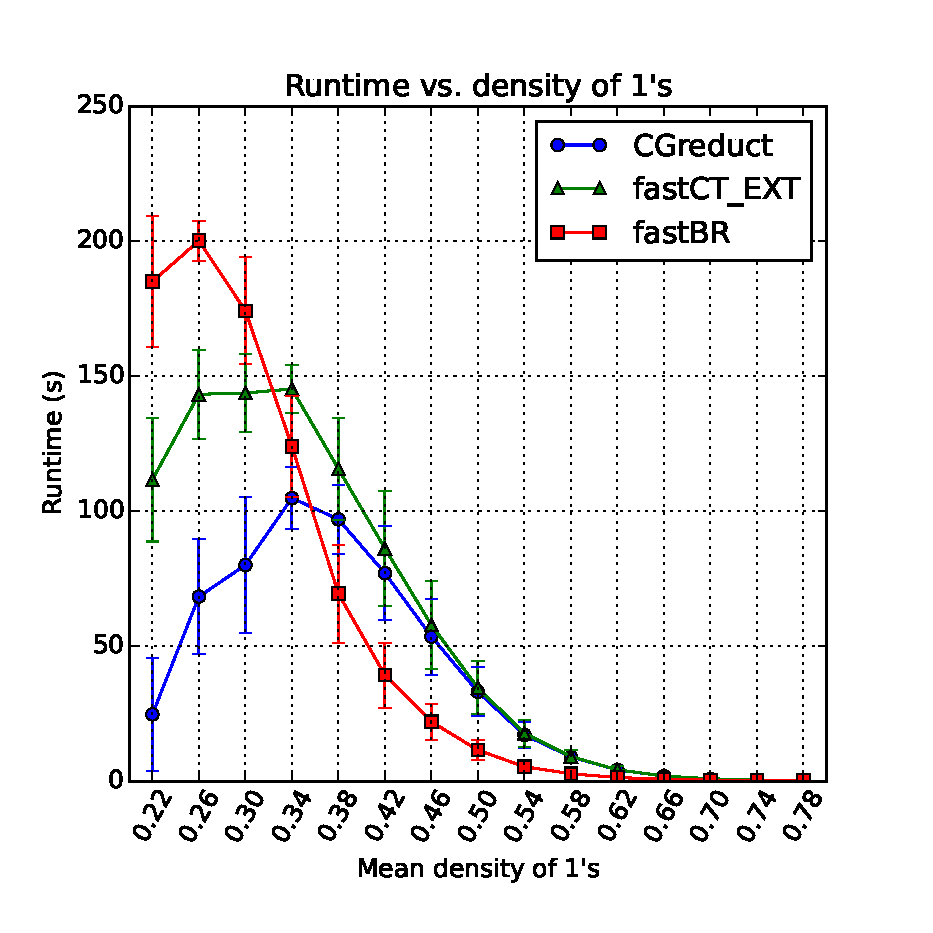
\includegraphics[height=8cm]{overal.eps}
		\end{center}
		\caption{Average algorithms' runtime vs. density of 1's for all synthetic \textit{SBDMs}.}
		\label{fig:scattDensity}
	\end{figure}	

	For clarity purposes, the 500 matrices were split into 15 groups discretizing the range of densities, each group having approximately 33 \textit{SBDMs}. Figure~\ref{fig:scattDensity} shows the average runtime of all  matrices in each group for the three algorithms, as a function of the density of 1's in the synthetic \textit{SBDMs}. In this figure, the vertical bars show the standard deviation of each bin. 
		
	From Figure~\ref{fig:scattDensity}, we can see that the fastest algorithm for matrices with density under or equal 0.35 was GCreduct, fast--BR was the fastest for matrices with density between 0.35 and 0.65, and the three algorithms presented similar performance for matrices with density above 0.65. The fact that high density \textit{SBDMs} do not constitute a complex computational task for reduct computation \citep{Rojas12} is clearly visible in Figure~\ref{fig:scattDensity}. For this reason, a detailed analysis in this region lacks of relevance.
		
	In order to explain the line delimiting those \textit{SBDMs} for which GCreduct is faster than fast--BR (densities under 0.35), we must go deeply into the main difference between these algorithms. In GCreduct, we compute the exclusion mask and evaluate the attribute exclusion, using proposition~\ref{prop:exclude}, for those candidates detected as super-reducts; in order to verify whether they are reducts. In fast--BR, on the other hand, the proposition~\ref{prop:exclude} is evaluated for each candidate with a contributing attribute. The evaluation of the attribute exclusion has the highest computational complexity in the algorithm ($\Theta (nm)$). The attribute exclusion occurs when there is at least one column in the sub-matrix of the \textit{SBDM}, considering only the attributes in the current candidate, that can be removed without increasing the number of zero rows in this sub-matrix. The exclusion is more frequent in matrices with a higher density of 1's, since it is given by cumulative OR operations. The higher cost of candidate evaluation in fast--BR pays off for \textit{SBDMs} with higher densities (the limit identified from our experiment is 0.35), because supersets of candidates with attribute exclusion are excluded from subsequent evaluations. Take for instance the extreme case of the identity matrix, where there is no exclusion at all, since every attribute is indispensable to form a reduct. For this kind of \textit{SBDMs}, GCreduct needs to evaluate as many candidates as fast--BR but the former makes a single verification for exclusion with the set of all attributes. On the other hand, fast--BR verifies the exclusion for each candidate, which leads to a higher computational cost.
	
	Friedman tests and post hoc Nemenyi-Damico-Wolfe-Dunn tests, show that GCreduct was significantly faster (\textit{p--value} $< 10^{-16}$) than fast--CT\_EXT for low (under 0.35) and medium (between 0.35 and 0.65) density matrices. 
%	For high density \textit{SBDMs} there was no significant difference (\textit{p--value} = 0.87) between these two algorithms. 
	In relation to fast--BR, GCreduct showed a significant runtime reduction (\textit{p--value} $< 10^{-16}$) for low density matrices while it was significantly slower (\textit{p--value} $< 10^{-16}$) for medium density matrices. 
%	GCreduct presented a significant improvement (\textit{p--value} = 0.0068) over fast--BR in the overall analysis, due to the higher runtime taken by low density matrices. 
	From this analysis, we conclude that GCreduct is the best algorithm for low density matrices; while fast--BR is the best for medium density matrices. For high (over 0.65) density matrices any algorithm can be used since, as we already commented, computing reducts of this kind of matrices does not constitute a complex computational task. Moreover, from these conclusions, a great advantage can be taken of selecting the appropriate algorithm for each information system, as it will be shown in the next subsection. 
		
	\begin{table}[htb]
		\centering
		\caption{Fast--CText, GCreduct and Fast--BR runtimes in seconds for standard information systems. Sorted by \textit{SBDM} density.}
		\label{tab:density}
		\begin{tabular}{|l|c|r|r|r|}
			\hline
			\multicolumn{1}{|c|}{Information}  && Fast--CText & \multicolumn{1}{c|}{Gcreduct} & \multicolumn{1}{c|}{Fast--BR}  \\
			\multicolumn{1}{|c|}{system}       & Density & runtime (s) & runtime (s)  & runtime (s)  \\
			\hline
			Chess (kr-vs-kp)          & 0.03    & 7.45          & \textbf{$<$0.01} & 0.02            \\
			Keyword-activity          & 0.04    & 1.22          & \textbf{0.42}    & 0.90            \\
			Connect-4                 & 0.05    & 12876.67      & \textbf{44.23}   & 160.61          \\
			QSAR-biodeg               & 0.12    & 0.75          & \textbf{0.19}    & 0.33            \\
			Landsat (train)           & 0.33    & 23797.99      & \textbf{9949.31} & 17732.49        \\
			Dermatology               & 0.34    & 16.02         & 12.25            & \textbf{4.62}   \\
			Credit-g                  & 0.35    & \textbf{0.05} & 0.06             & 0.12            \\
			Flags                     & 0.35    & 1.00          & \textbf{0.74}    & 1.06            \\
			Diabetes                  & 0.38    & 86.99         & \textbf{19.48}   & 23.37           \\
			Student-por               & 0.41    & 1874.57       & 1657.90          & \textbf{161.35} \\
			Sponge                    & 0.42    & 0.63          & 0.58             & \textbf{0.14}   \\
			Student-mat               & 0.43    & 1003.87       & 929.46           & \textbf{81.82}  \\
			Lung-cancer               & 0.47    & 188.20        & 133.43           & \textbf{7.34}   \\
			Waveform                  & 0.50    & 2.11          & 1.88             & \textbf{1.64}   \\
			Cylinder-bands            & 0.55    & 5.03          & 4.59             & \textbf{0.53}   \\
			\hline
		\end{tabular}
	\end{table}
	
	In Table~\ref{tab:density} we included the density of 1's of \textit{SBDMs} to the results from Table~\ref{tab:java}. We also sorted the information systems in Table~\ref{tab:density} in ascending order of the density of 1's in their associated \textit{SBDM}. Although this is a small heterogeneous sample, the rule obtained from synthetic data can be verified in this table. For information systems with densities close to the boundary of 0.35 we cannot conclude a fastest algorithm as it can be seen in Table~\ref{tab:java}. However, for those information systems which have a \textit{SBDM} with density clearly under 0.35, GCreduct performed faster. In the same way, fast-BR performed faster for those information systems with density clearly above 0.35.

\section{Conclusions}\label{conclusions}
	In this work, we presented a new algorithm, GCreduct, for reduct computation. In our proposed algorithm, the search space is traversed evaluating some candidate subsets and discarding others, based on previous evaluations. Algorithms reported in the literature use operations with a high cost for candidate evaluation in order to reduce the number of evaluated candidates. The main contribution of our proposal, on the other hand, is the use of simpler operations for candidate evaluation, based on the pruning properties of gap elimination and attribute contribution, which allows to reduce the required runtime. 
	
	After conducting a series of experiments over synthetic and standard information systems, we can conclude that GCreduct performs faster than all other recent reported alternatives in a specific kind of information systems. This result provides an instrument to select the proper algorithm for a determined information system, based on its density. Further studies should be devoted to explore the relation found between the fastest algorithm for reduct computation of an information system, and the density of 1's of the \textit{SBDM} associated to it. Furthermore, the feasibility of the introduction of this relation as a preprocessing stage for reduct computation, should be also studied.
	
%-------------------------------------------------------------------------------
% Bibliography
%-------------------------------------------------------------------------------
\newpage 
\bibliography{mybib}{}
\bibliographystyle{authordate1}
\end{document}
